\documentclass[
      12pt,
        ]{article}



% --- type and typeface? -----------------------
%% if scaleable font error:
\usepackage[T1]{fontenc}
\usepackage{lmodern}

% strikethrough text
\usepackage[normalem]{ulem}

% input
\usepackage[utf8]{inputenc}

% typography
\usepackage{microtype}


\usepackage[T1]{fontenc}


% text block
\usepackage{setspace}
\usepackage[ 
              left = 1in,top = 1in,right = 1in,bottom = 1in 
            ]{geometry}

\usepackage{enumitem}
  \setlist{noitemsep}



% decimal numbering for appendix figs and tabs


% Deletes section counters
%\setcounter{secnumdepth}{0}







  \usepackage{longtable, booktabs}

  \usepackage{graphicx,grffile}
  % Scale images; don't overflow page margins by default.
  % Still possible explicate \includegraphics[width, height, ...]{}
  \makeatletter
    \def\maxwidth{\ifdim\Gin@nat@width>\linewidth\linewidth\else\Gin@nat@width\fi}
    \def\maxheight{\ifdim\Gin@nat@height>\textheight\textheight\else\Gin@nat@height\fi}
  \makeatother 
  \setkeys{Gin}{width=\maxwidth,height=\maxheight,keepaspectratio}








  \usepackage{natbib}
  \bibliographystyle{assets/apsr}
  % protect underscores in most circumstances
  \usepackage[strings]{underscore} 


% 

% \newtheorem{hypothesis}{Hypothesis}

\makeatletter
  \@ifpackageloaded{hyperref}{}{%
    \ifxetex
      % page size defined by xetex
      % unicode breaks when used with xetex
      \PassOptionsToPackage{hyphens}{url}\usepackage[setpagesize = false, 
                                                     unicode = false, 
                                                     xetex]{hyperref}
    \else
      \PassOptionsToPackage{hyphens}{url}\usepackage[unicode = true]{hyperref}
    \fi
  }

  \@ifpackageloaded{color}{
    \PassOptionsToPackage{usenames,dvipsnames}{color}
  }{
    \usepackage[usenames,dvipsnames]{color}
  }
\makeatother

\hypersetup{breaklinks = true,
            bookmarks = true,
            pdfauthor = {Devin Judge-Lord (University of Wisconsin-Madison)},
             pdfkeywords  =  {},  
            pdftitle = {APSA Dissertation Research Improvement Grant Template},
            colorlinks = false,
            citecolor = blue,
            urlcolor = blue,
            linkcolor = magenta,
            pdfborder = {0 0 0}}

% \urlstyle{same}  % don't use monospace font for urls


% set default figure placement to htbp
\makeatletter
  \def\fps@figure{hbtp}
\makeatother

  \usepackage{booktabs}
  \usepackage{longtable}
  \usepackage{array}
  \usepackage{multirow}
  \usepackage{wrapfig}
  \usepackage{float}
  \usepackage{colortbl}
  \usepackage{pdflscape}
  \usepackage{tabu}
  \usepackage{threeparttable}
  \usepackage{threeparttablex}
  \usepackage[normalem]{ulem}
  \usepackage{makecell}

% optional footnotes as endnotes


% ----- Pandoc wants this tightlist command ----------
\providecommand{\tightlist}{
  \setlength{\itemsep}{0pt}
  \setlength{\parskip}{0pt}
}





% --- title & section styles -----------------------


% title, author, date
  \title{APSA Dissertation Research Improvement Grant Template}
 

  \author{ % author, option footnote, optional affiliation
            Devin Judge-Lord  \\ \emph{University of Wisconsin-Madison} 
            }

% auto-format date?
  \date{\today}


% abstract
\usepackage{abstract}
  \renewcommand{\abstractname}{}    % clear the title
  \renewcommand{\absnamepos}{empty} % originally center

  \newcommand*{\authorfont}{\sffamily\selectfont}


% section titles
% \usepackage[small, bf, sc]{titlesec}
  % \titleformat*{\subsection}{\itshape}
  %\titleformat*{\subsubsection}{\itshape} 
  %\titleformat*{\paragraph}{\itshape} 
  %\titleformat*{\subparagraph}{\itshape}

% \newcommand{\sectionbreak}{\clearpage}






\begin{document}
 

% --- PAGE: title and abstract -----------------------

  \maketitle

% \pagenumbering{gobble}




% --- PAGE: contents -----------------------





% --- PAGE: body -----------------------



\noindent 
 
   
   
\hypertarget{section}{%
\subsection{}\label{section}}

\begin{quote}
Fork this repository at \url{https://github.com/judgelord/ddrig}. (Or download just the \href{https://judgelord.github.io/ddrig/app.docx}{.docx} or \href{https://judgelord.github.io/ddrig/app.tex}{.tex} template if you don't use bookdown.)
\end{quote}

\begin{quote}
If you choose to \href{https://github.blog/2016-08-17-simpler-github-pages-publishing/}{publish} your new ddrig repository, your friends and advisors will be able to read your draft proposal as a web page or download it as a .docx or .pdf at the link above.
\end{quote}

\begin{center}\rule{0.5\linewidth}{0.5pt}\end{center}

See the wonderful bookdown documentation at \url{https://bookdown.org/}.

\begin{center}\rule{0.5\linewidth}{0.5pt}\end{center}

The \texttt{/assets} folder contains some key tools:

\begin{itemize}
\tightlist
\item
  \texttt{apsr.bst} formats your citations
\item
  LaTeX is formatted with \texttt{article-template.tex} adapted from \url{https://github.com/svmiller/svm-r-markdown-templates}
\item
  \texttt{clean-bib.R} removes any problematic special characters from a .bib file (e.g., one exported from Mendeley or Zotero)
\end{itemize}

\texttt{/docs} is where the .html, .pdf, and .docx output will appear

\texttt{/figs} is where to put figures you want to include

\newpage

\hypertarget{summary}{%
\section{Summary}\label{summary}}

\begin{quote}
No longer than 1 page, single-spaced
\end{quote}

\begin{quote}
The proposal summary should be a succinct overview of the project, including the central research \emph{question}, a brief note on how the project fits with \emph{existing research} on the issue, a short overview of the research \emph{plan}, and an indication of \emph{how the grant is expected to improve the overall dissertation}.
\end{quote}

\newpage

\hypertarget{project-description-and-research-plan}{%
\section{Project description and research plan}\label{project-description-and-research-plan}}

\begin{quote}
No longer than 15 pages, single-spaced
\end{quote}

\begin{quote}
The project description and research plan should provide a full description of the \emph{overall research project}, as well as a well-developed summary of \emph{how the grant-supported activities will improve the overall dissertation research}. The project description should explicitly address the intellectual merit, and broader impact of the overall dissertation research, as well as how the \emph{additional activities} supported by the grant will expand either or both. This should include a clear description of the research question and how it fits into the existing literature, along with a well-developed research plan and \emph{timeline}.
\end{quote}

\begin{quote}
All references cited in the project description and research plan should be included in a separate citation page, which will not count against the page limit.
\end{quote}

\setcounter{page}{1}

\hypertarget{the-intellectual-merit-of-studying-a}{%
\subsection{The intellectual merit of studying A}\label{the-intellectual-merit-of-studying-a}}

``The heavenly chorus sings with an upper-class accent'' \citep{Schattschneider1975}.

\hypertarget{the-intellectual-merit-of-studying-b}{%
\subsection{The intellectual merit of studying B}\label{the-intellectual-merit-of-studying-b}}

See Figure \ref{fig:hello-world}.

\begin{figure}
\centering
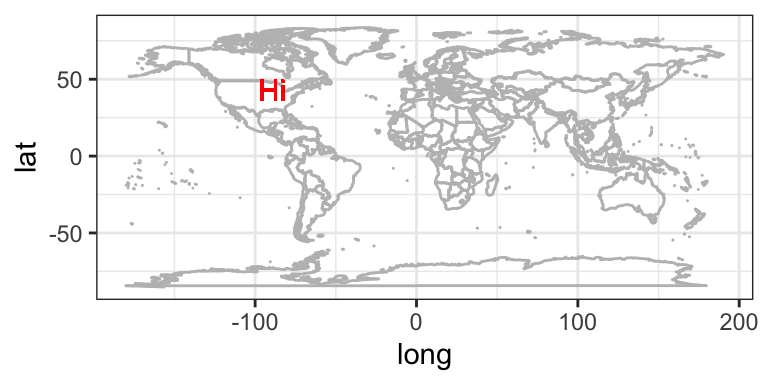
\includegraphics{figs/hello-world-1.pdf}
\caption{\label{fig:hello-world}Hello World!}
\end{figure}

\hypertarget{the-intellectual-merit-of-studying-c}{%
\subsection{The intellectual merit of studying C}\label{the-intellectual-merit-of-studying-c}}

Lorem ipsum dolor sit amet, consectetur adipiscing elit.

\hypertarget{really-really-meritorious}{%
\subsubsection{Really, really meritorious!}\label{really-really-meritorious}}

Lorem ipsum dolor sit amet, consectetur adipiscing elit!

\hypertarget{the-broader-impacts-of-research-and-data-on-x}{%
\subsection{The broader impacts of research and data on X}\label{the-broader-impacts-of-research-and-data-on-x}}

Lorem ipsum dolor sit amet, consectetur adipiscing elit.

\hypertarget{the-broader-impacts-of-y}{%
\subsection{The broader impacts of Y}\label{the-broader-impacts-of-y}}

Lorem ipsum dolor sit amet, consectetur adipiscing elit.

\hypertarget{the-broader-impacts-of-z}{%
\subsection{The broader impacts of Z}\label{the-broader-impacts-of-z}}

Lorem ipsum dolor sit amet, consectetur adipiscing elit.

\hypertarget{timeline}{%
\subsection{Timeline}\label{timeline}}

Lorem ipsum dolor sit amet, consectetur adipiscing elit.

\newpage

\hypertarget{current-and-pending-sources-of-support}{%
\section{Current and pending sources of support}\label{current-and-pending-sources-of-support}}

\begin{quote}
Proposals will be required to indicate any current and pending grant support for the research scholar, including but not limited to any research funding related to the relevant dissertation project. Proposals will also be required to disclose any past forms of support for the dissertation project, including previous NSF DDRIG awards.
\end{quote}

\newpage

\hypertarget{professional-development-plan}{%
\section{Professional development plan}\label{professional-development-plan}}

\begin{quote}
\sout{No longer than 1 page, single-spaced} 500 words
\end{quote}

\begin{quote}
Proposals must include a brief professional development plan describing steps the research scholar plans to take to advance \emph{his or her} research career. This should include an explanation of how the research scholar envisions the dissertation project fitting into an expected \emph{long-term research agenda} as well as an indication of a professional development opportunity (or opportunities) at which the research could be \emph{presented} and improved. In addition, the professional development plan may identify further \emph{training} that will enhance the research scholar's long-term research agenda, plans and opportunities for creating or joining \emph{professional networks}, and plans and opportunities for \emph{sharing research in public spaces}.
\end{quote}

\textbf{Professional Development and Service}

Lorem ipsum dolor sit amet, consectetur adipiscing elit. Praesent vel mi lacus. Aenean facilisis vehicula elit ut faucibus. Vestibulum nec maximus odio. Fusce id sapien in sapien fermentum bibendum. Proin pellentesque vehicula ligula, eget varius ex facilisis ut. Nulla in tellus at metus porttitor eleifend a ut nulla. In hac habitasse platea dictumst. Nam nisl mi, vehicula ac quam ac, accumsan dictum nisi. Nullam suscipit justo dolor, ut pharetra arcu pulvinar a. Curabitur in odio sit amet metus consectetur faucibus. Aliquam vitae ligula sem. Curabitur feugiat velit libero, non vestibulum ligula ornare at. Interdum et malesuada fames ac ante ipsum primis in faucibus. Duis eget vehicula ligula. Phasellus in quam eget mauris feugiat sollicitudin id sed eros.

\textbf{Publicising Resaerch}

Lorem ipsum dolor sit amet, consectetur adipiscing elit. Praesent vel mi lacus. Aenean facilisis vehicula elit ut faucibus. Vestibulum nec maximus odio. Fusce id sapien in sapien fermentum bibendum. Proin pellentesque vehicula ligula, eget varius ex facilisis ut. Nulla in tellus at metus porttitor eleifend a ut nulla. In hac habitasse platea dictumst. Nam nisl mi, vehicula ac quam ac, accumsan dictum nisi. Nullam suscipit justo dolor, ut pharetra arcu pulvinar a. Curabitur in odio sit amet metus consectetur faucibus. Aliquam vitae ligula sem. Curabitur feugiat velit libero, non vestibulum ligula ornare at. Interdum et malesuada fames ac ante ipsum primis in faucibus. Duis eget vehicula ligula. Phasellus in quam eget mauris feugiat sollicitudin id sed eros.

\textbf{Future Research}

Lorem ipsum dolor sit amet, consectetur adipiscing elit. Praesent vel mi lacus. Aenean facilisis vehicula elit ut faucibus. Vestibulum nec maximus odio. Fusce id sapien in sapien fermentum bibendum. Proin pellentesque vehicula ligula, eget varius ex facilisis ut. Nulla in tellus at metus porttitor eleifend a ut nulla. In hac habitasse platea dictumst. Nam nisl mi, vehicula ac quam ac, accumsan dictum nisi. Nullam suscipit justo dolor, ut pharetra arcu pulvinar a. Curabitur in odio sit amet metus consectetur faucibus. Aliquam vitae ligula sem. Curabitur feugiat velit libero, non vestibulum ligula ornare at. Interdum et malesuada fames ac ante ipsum primis in faucibus. Duis eget vehicula ligula. Phasellus in quam eget mauris feugiat sollicitudin id sed eros.

\newpage

\hypertarget{biographical-sketch}{%
\section{Biographical sketch}\label{biographical-sketch}}

\begin{quote}
No longer than 2 pages, single-spaced
\end{quote}

\begin{quote}
The biographical sketch must include: relevant professional training, including undergraduate and graduate education and supplemental training programs; any appointments or accomplishments, including service and teaching obligations, that may speak to the research scholar's professional development and ability to conduct the proposed research; and, any published or in-progress papers or products that speak to the research scholar's research agenda and ability to conduct the proposed research. Biographical sketches may be in narrative form or in the form of a curriculum vitae.
\end{quote}

\newpage

\hypertarget{budget-justification}{%
\section{Budget justification}\label{budget-justification}}

\begin{quote}
3 Pages
\end{quote}

\begin{quote}
Proposals must include a proposed budget, which will detail the specific expenses for which the award funds will be used, including any costs associated with research materials or equipment, research assistance, or travel. Proposed budgets should also include an expected timeline for expenditures and indicate whether the research scholar expects the grant to be active for one year or two years.
\end{quote}

\begin{quote}
APSA Doctoral Dissertation Improvement Grants will cover only direct costs for research activities. The grant is not intended to provide the full costs of a student's doctoral dissertation research. Project budgets should be developed at scales appropriate for the work to be conducted and may only include costs directly associated with the conduct of dissertation research. For APSA grants, overhead or indirect costs are not considered allowable expenses.
\end{quote}

\begin{quote}
The grant is intended to provide funding for research costs not normally covered by the grantee's university. Examples of the kinds of expenses that may be included in a proposal budget are the following:
\end{quote}

\begin{itemize}
\tightlist
\item
  costs for data-collection activities, including the conduct of surveys, questionnaires, and/or focus groups or the -purchase of extant data\\
\item
  costs for equipment necessary for the conduct of the project that will be devoted to the project over the duration of the award\\
\item
  costs for payments to research subjects and/or informants
\item
  analysis and research services not otherwise available
\end{itemize}

\begin{quote}
Along with the proposed budget itself, proposals must include a budget justification, explaining and justifying each budget line. The budget justification should be no longer than three pages single spaced.
\end{quote}

\newpage

\hypertarget{data-management-plan}{%
\section{Data management plan}\label{data-management-plan}}

\begin{quote}
\sout{No longer than 2 pages, single-spaced} 1000 words
\end{quote}

\begin{quote}
Proposals will require a data management plan that describes the data that will be generated by the research, how the data will be managed, secured, and shared, and other pertinent information about the content and handling of the data.
\end{quote}

\emph{Data, software, and other materials to be produced in the course of the project}

Documentation on how to use the software and access the data will be avaiable on GitHub.

\emph{Standards to be used for data and metadata format and content}

All datasets will be available in .Rdata and SQL format.

\emph{Policies for access and sharing}

All data will be publically available on GitHub.

Both R packages will be hosted as public repositories on GitHub so that anyone can contribute to their source code.

\emph{Policies and provisions for re-use, re-distribution, and the production of derivatives}

All data and R packages created through this project will be avaible for re-use under the Geneal Public License, GPL-3 standard.

\emph{Plans for archiving data, samples, and other research products, and for preservation of access to them}

Both R packages and most data will be available on GitHub.com.

\newpage

\hypertarget{ethics}{%
\section{Ethics}\label{ethics}}

\begin{quote}
\sout{No longer than 1 page, single-spaced} 500 words
\end{quote}

\begin{quote}
APSA is committed to promoting and supporting the highest levels of research and professional ethics. applicants will be required to provide a statement affirming their commitment to research ethics, and describing the application of the principles of research ethics in their projects. This should include addressing questions around ethical implementation of human subjects research as well as whether the applicant knows of any potential issues regarding conflicts of interest or scientific integrity for their projects. This may overlap with issues addressed in the data management plan, but most issues around the ethical handling of data should be covered in the data management plan. In developing this statement it may be useful to refer to the APSA Ethics Guide and Principles and Guidance for Human Subjects Research.
\end{quote}

\begin{quote}
Applicants with projects involving human subjects must provide documentation indicating that they have applied for or already gained IRB approval or exemption for their research plan (for example, the letter of approval or exemption from the IRB or a letter or email confirming submission of an application to the IRB). Applicants who submit documentation of having applied for IRB approval will be asked to submit verification of IRB approval upon receipt of such approval.
\end{quote}

In line with the \emph{APSA Guide to Professional in Political Science} (especially principles 3, 5, and 10), I will gratefully acknowledge support from the NSF APSA DDRIG and all Research Assistants who wish to be acknowledged in all resulting published work, including replication data and software.

With respect to principle 6. the data and code to replicate all analysis will be available on GitHub.com.

\newpage
% --- PAGE: endnotes -----------------------
% --- PAGE: refs -----------------------
\newpage
\singlespacing 
          \bibliography{assets/dissertation.bib} 
   

\end{document}
